\documentclass[11pt]{article}
\usepackage[a4paper,margin=2.4cm]{geometry}
\usepackage{amsmath}
\usepackage{graphicx}
\usepackage{booktabs}
\usepackage{siunitx}
\usepackage{caption}
\usepackage{xcolor}
\usepackage{hyperref}
\definecolor{linknavy}{RGB}{20,70,130}
\hypersetup{colorlinks=true, urlcolor=linknavy, linkcolor=black, citecolor=black}
\captionsetup{font=small,labelfont=bf}
\sisetup{detect-all, exponent-product=\times, separate-uncertainty=true}
\setlength{\parskip}{0.4em}
\setlength{\parindent}{0pt}

\newcommand{\De}{D_{\mathrm{e}}}
\newcommand{\Df}{D_{\mathrm{f}}}
\newcommand{\Nexc}{N_{\mathrm{exc}}}

\title{What the $n_\infty$ lifetime fit determines,\\ and the truncation bias on
$\De/\Df$}
\author{Joseph J. Thiebes}
\date{\today}

\begin{document}

{\large\bfseries What the $n_\infty$ lifetime fit determines, and the truncation
bias on $\De/\Df$}\\[4pt]
{\small Joseph Thiebes \quad\textbar\quad working note, $n_\infty$ diffusion
analysis \quad\textbar\quad \today}\par
\vspace{1.1em}

\noindent
Two questions came up in the $n_\infty$ analysis. This note answers both from the
data.
\begin{enumerate}\itemsep2pt
\item What does the global multi-fluence lifetime fit determine? It pins down
three rates: how fast excitons recombine ($\nu$), how fast carriers are trapped
($\lambda$), and how fast trapped charge decays ($\gamma$). It does not pin down
the free-charge bimolecular rate $\rho$. The Saha equilibrium ties $\rho$ to
$\nu$ so tightly that the fit sees only their sum.
\item Does the measurement (truncation) bias distort the $\De/\Df$ fit? No. It is
negligible against the $\De/\Df$ error bars.
\end{enumerate}
All numbers come from the three $n_\infty$ TPLM fluences,
$\Nexc = \SI{5.5e17}{}, \SI{3.1e18}{}, \SI{7.2e19}{cm^{-3}}$.

\section{What the global lifetime fit determines}

To learn which rates the three decays pin down, we fit all three PL curves at
once with one shared rate set ($\nu$, $\rho$, $\lambda$, $\gamma$, and the trap
emission ratio $q_{\mathrm{trap}}$, the share of the light that comes from
trapped charge); only $\Nexc$ differs between the curves. This shared-rate fit
reproduces the overall decay shape (Fig.~\ref{fig:globalfit}). It under-fits the
late-time tail at the two lower fluences. That tail constrains the trap
parameters ($\gamma$ and $q_{\mathrm{trap}}$), not the result below, so we set it
aside here.

\begin{figure}[ht]
\centering
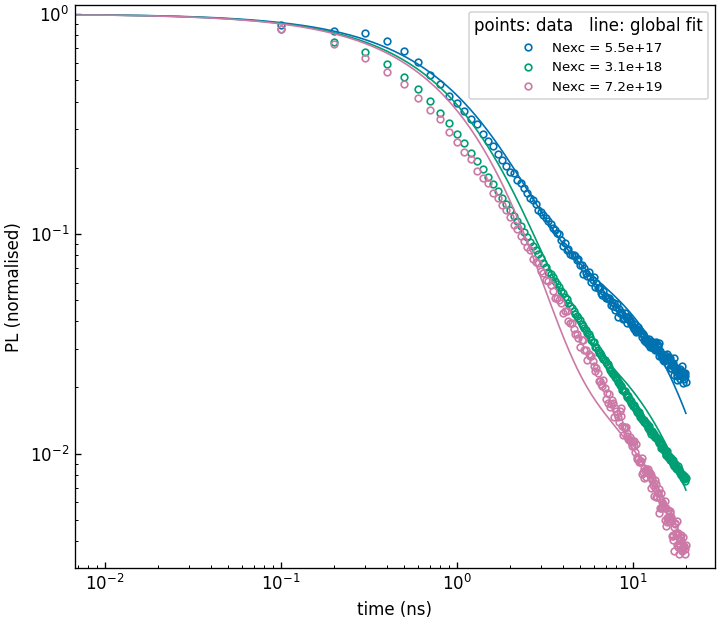
\includegraphics[width=0.62\textwidth]{n_inf_lifetime_global_fit.png}
\caption{Global multi-fluence fit. Points: data; lines: the shared-rate fit. The
overall decay is reproduced; the late-time tail at the two lower fluences is
under-fit.}
\label{fig:globalfit}
\end{figure}

To find which rates the data determine, we test each rate one at a time. We fix
the rate at a series of values; at each value we re-fit the other rates and
measure how well the fit matches the data. That measure is the sum of squared
residuals (SSR): for each data point we take the gap between the fitted curve and
the data, square it, and add the squares over all points. (We use the logarithm
of the PL, because the decay spans several decades, so we compare ratios rather
than absolute differences.) A small SSR means a good fit.
This recipe (fix one rate, re-fit the rest, read the SSR) is the
profile-likelihood method, the same method used for the $\De/\Df$ error bars. It
uses no random sampling, so it returns the same answer every run.

We then read each rate from the shape of its SSR. A clear minimum means the rate
is determined; a flat profile means it is not. The width of the minimum sets the
error bar: a value is still acceptable as long as forcing the rate there barely
worsens the fit, and ``barely'' is set by the size of the data's own scatter.
That scatter is the residual variance, $s^2 = \mathrm{SSR}_{\min}/(N-p) =
\SI{4.2e-3}{}$, where $N = 600$ is the number of data points and $p = 6$ the
number of fitted rates. The $\sim\!1\sigma$ interval for a rate is the range over
which its SSR rises by no more than $s^2$ above the minimum
(Fig.~\ref{fig:profile}).

\begin{figure}[ht]
\centering
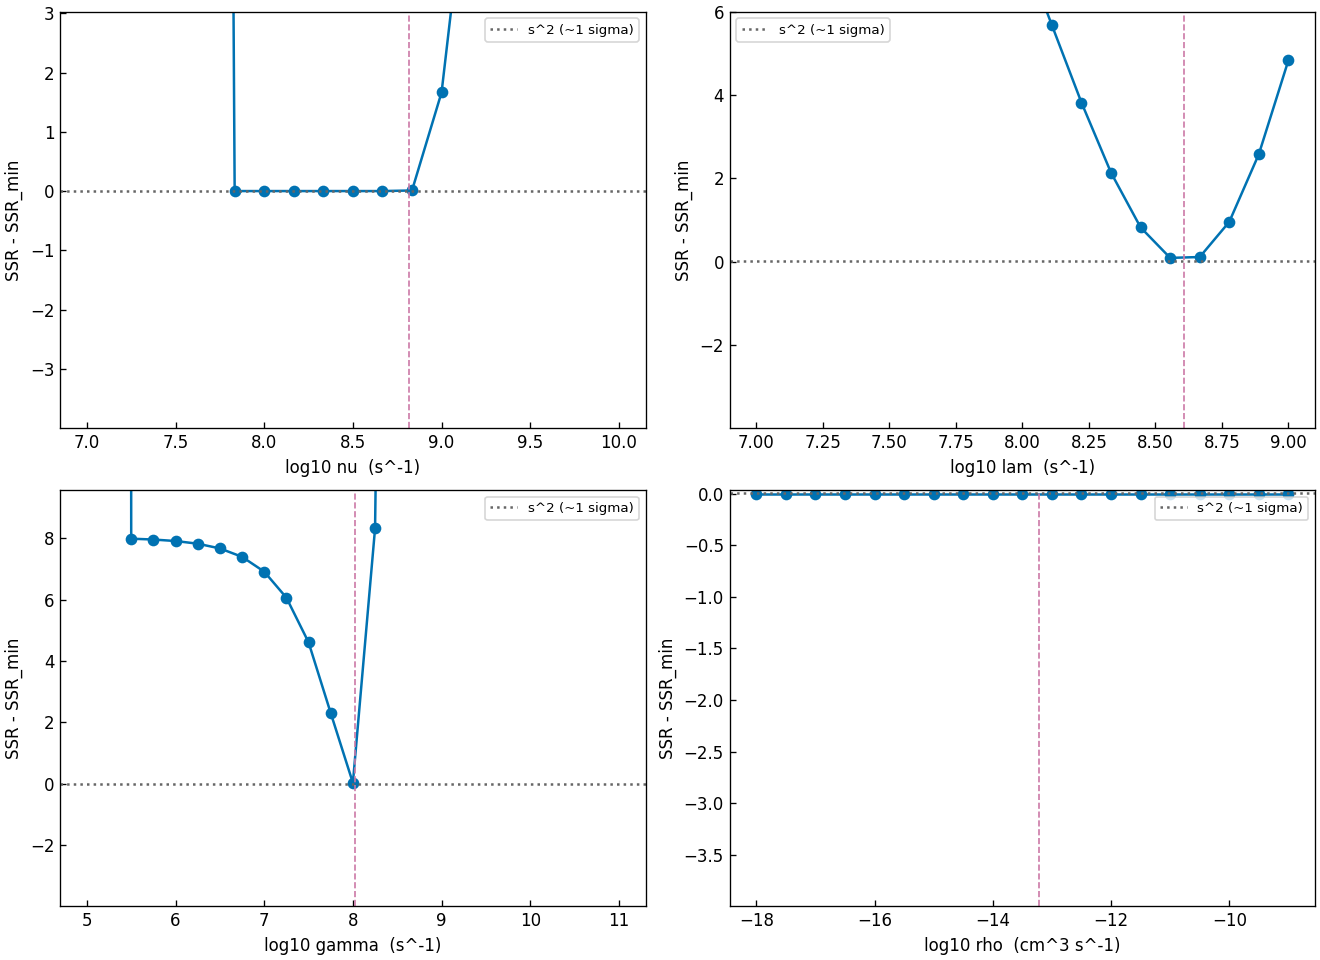
\includegraphics[width=0.92\textwidth]{n_inf_lifetime_profile_ci.png}
\caption{Profile likelihood of each rate ($\mathrm{SSR}$ minus its minimum,
versus the value the rate is fixed at; dotted line: the $s^2$ threshold; dashed
line: the best fit). The shapes tell the story: $\nu$ is a plateau with a hard
lower wall, so it is bounded but not pinned to one value; $\lambda$ is a clean
well (well determined); $\gamma$ has a minimum near \SI{1e8}{s^{-1}}; $\rho$ is
flat, so the data do not determine it.}
\label{fig:profile}
\end{figure}

\begin{table}[ht]
\centering
\caption{What the three decays determine. Rates in \si{s^{-1}}; $\rho$ in
\si{cm^3/s}.}
\label{tab:rates}
\begin{tabular}{lll}
\toprule
rate & meaning & result \\
\midrule
$\nu$     & exciton recombination   & determined as a bracket, $\sim[0.8,6]\times10^{8}$; rejects $>10^{9}$ \\
$\lambda$ & carrier trapping        & determined, $\SI{4.06e8}{}$, $1\sigma$ $[3.96,4.17]\times10^{8}$ \\
$\gamma$  & trapped-charge decay    & determined, $\sim\!\SI{1e8}{}$ (trap lifetime $\sim$\SI{10}{ns}) \\
$\rho$    & free-charge bimolecular & \textbf{not determined} (flat profile, $10^{-18}$ to $10^{-9}$) \\
\bottomrule
\end{tabular}
\end{table}

The results are in Table~\ref{tab:rates}. $\nu$ is bounded, not pinned to a
point. Its SSR is a plateau: equally good for any $\nu$ across a wide band,
sharply worse below about $\SI{8e7}{s^{-1}}$, and gradually worse above. So the
data place a firm floor under $\nu$ and a soft ceiling over it, rejecting
$\nu > \SI{1e9}{s^{-1}}$ and fencing it into roughly
$[0.8,6]\times10^{8}\,\si{s^{-1}}$. We call this a bracket: a range, not a single
value.

$\lambda$ is different. It has a clean minimum and is the best-determined rate:
$\lambda = \SI{4.06e8}{s^{-1}}$, with a formal $1\sigma$ interval
$[3.96, 4.17]\times10^{8}\,\si{s^{-1}}$ (half-width $2.6\%$, from a fine grid
around the minimum). One caution applies here above all. This interval assumes
the residuals are independent. They are not: a smooth decay makes neighbouring
residuals move together, so the true uncertainty on $\lambda$ is wider than
$2.6\%$.

\paragraph{Why the fit cannot determine $\rho$.}
The reason is exact, not a matter of weak signal, and it follows from the Saha
equilibrium. Two rates are degenerate when the data cannot tell them apart: any
increase in one can be cancelled by a decrease in the other, leaving the fitted
curves identical, so the fit pins only their combination. Here that combination
is $\nu + \rho A$, and the cause is a single algebraic fact.

The Saha free-charge fraction $x = 2/\!\big(\sqrt{4n/A + 1} + 1\big)$ obeys the
identity
\begin{equation}
1 - x = x^{2}\,n/A ,
\label{eq:saha}
\end{equation}
at every density (we checked this by algebra, and numerically to $\SI{6e-14}{}$).
Here $A$ is the Saha density scale, the density at which carriers are half
excitons and half free charge. The identity makes the two recombination channels
share one density shape: the exciton per-carrier rate $\nu(1-x)$ equals
$\nu\,x^{2}n/A$, a fixed multiple of the bimolecular per-carrier rate
$\rho\,x^{2}n$, with the ratio $\nu/(\rho A)$ constant at all densities
(Fig.~\ref{fig:saha}). The total recombination then collapses to one term,
\begin{equation}
\nu(1-x) + \rho\,x^{2}n = x^{2}n\,\big(\nu/A + \rho\big),
\end{equation}
so the data see only the sum $\nu + \rho A$. Changing the fluence cannot separate
$\nu$ from $\rho$, because the Saha coupling gives the two channels the same
dependence on density.

\begin{figure}[ht]
\centering
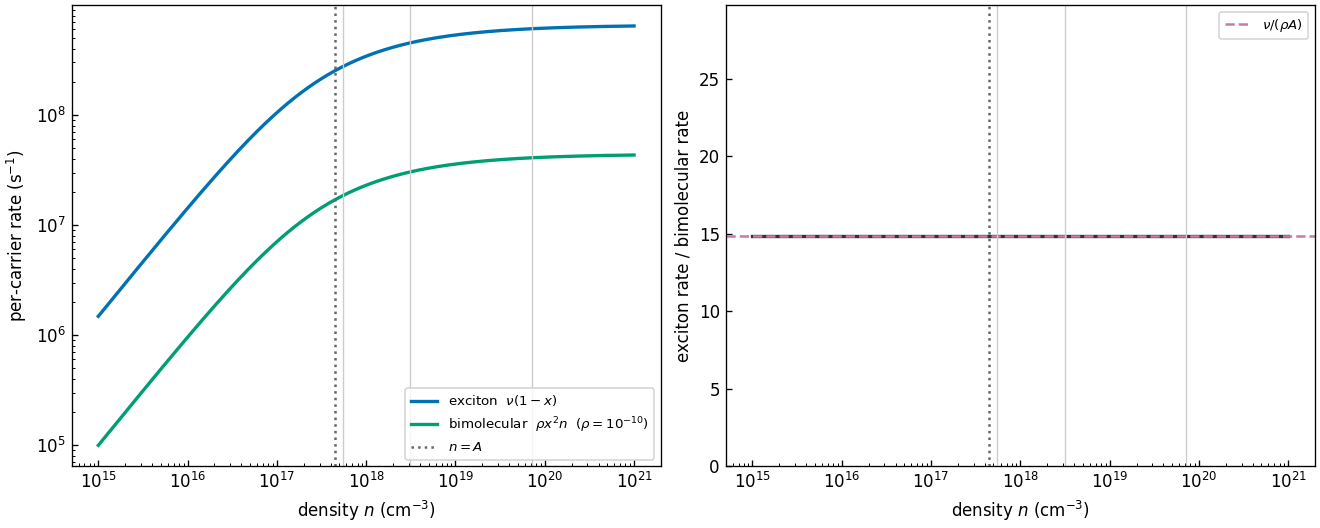
\includegraphics[width=0.92\textwidth]{n_inf_lifetime_saha_collapse.png}
\caption{The Saha exact proportionality. Left: the exciton and bimolecular
per-carrier rates versus density (parallel on the log axes). Right: their ratio,
flat at $\nu/(\rho A)$ across all densities. Dotted line: $n=A$; light lines: the
three measured fluences. The fit sees only $\nu + \rho A$.}
\label{fig:saha}
\end{figure}

The fit shows this directly (Fig.~\ref{fig:tradeoff}). When we fix $\rho$ at a
series of values and re-fit the rest, $\nu$ tracks $\nu_{\mathrm{eff}} - \rho A$
to four significant figures, the fit quality does not change, and $\lambda$ and
$\gamma$ do not move (they shift by less than $0.01\%$). The fit holds
$\nu + \rho A$ fixed and lets $\nu$ absorb the change. This continues until
$\rho A$ reaches $\nu$ (near $\rho = \SI{1.5e-9}{cm^3/s}$). There $\nu$ can no
longer compensate, and the fit breaks. Only $\nu$ trades against $\rho$; the trap
channel is not involved.

\begin{figure}[ht]
\centering
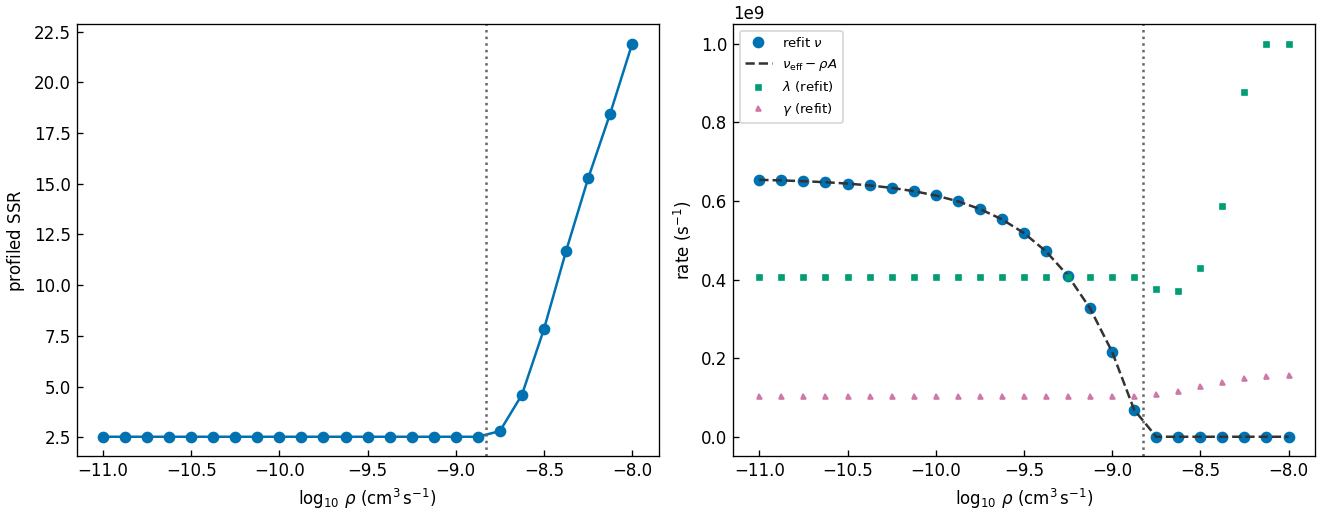
\includegraphics[width=0.92\textwidth]{n_inf_lifetime_rho_tradeoff.png}
\caption{The $\rho$--$\nu$ trade. Left: the fit quality (SSR) is flat until
$\rho A$ reaches $\nu$ (dotted line). Right: the re-fit $\nu$ tracks
$\nu_{\mathrm{eff}} - \rho A$ (dashed) while $\lambda$ and $\gamma$ stay fixed.
The data determine $\nu + \rho A$, not $\rho$.}
\label{fig:tradeoff}
\end{figure}

Free charges are not absent: the free-charge fraction at $t=0$ is $0.58$, $0.31$,
and $0.075$ across the three fluences. $\rho$ is invisible not because there are
no free charges, but because the Saha coupling makes its channel rise and fall
with density in step with the exciton channel. To separate the two, you need data
where they scale differently. One option is the low-density regime $n \ll A$:
there almost all charge is free ($x \to 1$), so the exciton channel vanishes and
the bimolecular channel returns to $\sim\!\rho n$, and the two no longer track
each other. Another is an independent measurement of the free charges, such as
their diffusion $\Df$.

\section{The truncation bias does not affect \texorpdfstring{$\De/\Df$}{De/Df}}

The width fit cannot return a negative width. So when the noise is large, the low
side of the fitted-width scatter is cut off and only the high side survives,
which pulls the average width upward. At low contrast-to-noise (CNR) the fitted
width is therefore biased high, and a width that is too large inflates the
late-time MSD. The question is whether that inflated MSD also inflates $\De/\Df$.

It does not. The reason is a single mechanism: low CNR causes both the bias and a
low fit weight. The $\De/\Df$ fit weights each frame by how trustworthy it is, so
a clean frame counts a lot and a noisy frame counts little (this is
inverse-variance weighting, with weight $\propto 1/\sigma^2$ and $\sigma$ the
per-frame MSD uncertainty). A low-CNR frame is at once biased (from the
truncation) and noisy (large $\sigma$), so the very frames that carry the bias
barely count. These are not two independent safeguards; they are one fact.

Table~\ref{tab:cnr} puts numbers on this. For each frame it lists the per-frame
CNR (measured with \href{https://github.com/thiebes/fft-cnr}{fft-cnr} on the
recorded profiles) next to that frame's weight in the fit, $w_i = 1/\sigma_i^2$, with the weights scaled to sum to one. The bias
is significant only near CNR $1$--$2$. In the two dimmer fluences, a quarter to
two-fifths of the frames fall in that range, but their summed weight is below
$\SI{2e-5}{}$ of the total. The weight-weighted mean CNR is $63$--$268$, so the
fit is carried by high-CNR frames, where there is no bias.

\begin{table}[ht]
\centering
\caption{Per-frame CNR and fit weight for the diffusion ($\De/\Df$) fit. The
bias-prone frames (CNR $<5$) carry a vanishing share of the fit weight.}
\label{tab:cnr}
{\small
\begin{tabular}{l c c c c}
\toprule
fluence & CNR & frames with & weight share of & weighted-mean \\
(\si{\micro J/cm^2}) & range & CNR $<5$ & those frames & CNR \\
\midrule
13.11  & $5.4$--$336$ & none        & ---            & 268 \\
2.298  & $1.8$--$137$ & $\sim 1/4$  & \num{1.9e-5}   & 85  \\
301.4  & $1.2$--$93$  & $\sim 2/5$  & \num{1.6e-5}   & 63  \\
\bottomrule
\end{tabular}
}
\end{table}

A simple bound follows. In a weighted average, a group of points that holds
weight fraction $w$ can move the result by at most $w$ times how wrong it is. The
bias-prone frames here hold $w < \SI{2e-5}{}$. Even if their widths were wrong by
an amount as large as the MSD itself (a deliberate worst case), they would move
$D$ by less than $\SI{2e-5}{}$ of its value. The reported
$\De = \SI{0.030 +- 0.026}{cm^2/s}$ has a relative error near $0.87$. So the shift
from the bias is about $\SI{4e4}{}$ times smaller than the error bar.

No truncation correction is needed on the diffusion fits. The limit on $\De/\Df$
is the degeneracy between $\De$ and $\Df$ (the large error bars), which the
profile-likelihood error analysis addresses, not the bias.

\section{What to report}

\begin{itemize}\itemsep2pt
\item Report $\nu$, $\lambda$, and $\gamma$ from the lifetime fit; the data
determine them.
\item Do not fit $\rho$ from the lifetime data. Fix it from the diffusion data or
the literature, or report it as unconstrained by the lifetime. Once $\rho$ is
fixed, the degeneracy is broken and $\nu$ is determined, so you can leave $\nu$
free rather than fixing it too.
\item Do not add a Meitner-Auger term ($-C\,n^{3}$). We tested it: its
coefficient runs to zero and the fit quality does not change with it on or off,
so the lifetime decays do not constrain it (the same kind of degeneracy as
$\rho$). Keep its bound near the literature value ($C \sim \SI{1e-28}{cm^6/s}$
for a lead halide), but do not trust a fitted value that sits at a bound or whose
profile is flat.
\item Choose the bounds for $\lambda$, $\gamma$, and $C$ from physical ranges,
wide enough that the best value sits inside. After fitting, check that no
parameter sits at its bound: a value pinned at a bound is set by the bound, not
the data. $\gamma$ showed this. A bound placed at its best value made $\gamma$
look pinned, and widening the bound fixed it.
\end{itemize}

\paragraph{Method.}
Lifetime identifiability: the shared-rate global fit, then a profile of each rate
(fix one, re-fit the rest with a local optimiser, read the SSR against the fixed
rate). Bias: the per-frame CNR from fft-cnr on the recorded profiles, against the
$\De/\Df$ fit weight $1/\sigma_i^2$ (the fit minimises
$\chi^2 = \sum_i [(\mathrm{MSD}^{\mathrm{sim}}_i - \mathrm{MSD}_i)/\sigma_i]^2$).
The analysis script (\texttt{lifetime\_identifiability.py}) regenerates every
figure here.

\end{document}
